\documentclass[__main__.tex]{subfiles}

\begin{document}

\section{Сеточное табулирование и корректное сплайновое аппроксимирование чебышёвского пространства непрерывных на отрезке (на двумерном брусе) функций}

\paragraph{Пункт А}

Здесь $Y_0 = \underline{C} \left([a;b],\mathbb{R}\right)$ и $A_{\left(\cdot\right)} = \left(A_k\right)_{\mathbb{N}}$ - схема равномерных сеток. Для наглядности, $A_k = \langle a=\tau_0, \tau_1,...,\tau_k=b \rangle$, то есть $\left|A_k\right|=k+1$ и $stp\left(A_k\right)=\frac{b-a}{k}=h=h_k$.

Таким образом индуцируется сеточное табулирование $\hat{A}_{\left(\cdot\right)}=\left(\hat{A}_k\right)_{\mathbb{N}}$ пространства $Y_0$, где $\hat{A}_k \in Hom_c\left(Y_0,{}^>\underline{\mathbb{R}}^{k+1}=\underline{\upsilon}_{\left(k\right)}\right)$ - эпиморфизм и $\| \hat{A}_k \| = 1$ для $k \in \mathbb{N}$.

В качестве базы аппроксимирования $H_{\left(\cdot\right)} = \left(H_k\right)_{\mathbb{N}}$, согласованной с сеточным табулированием $\hat{A}_{\left(\cdot\right)}$ выбирается сплайновая база, где $H_k = \left(spl_1 \left(A_k; {}^> e_1\right),spl_1 \left(A_k; {}^> e_2\right),...,spl_1\left(A_k;{}^> e_{k+1}\right)\right)$ и $\left({}^> e_1; {}^>e_2,...,{}^>e_{k+1}\right)$ - стандартный базис ${}^>\mathbb{R}^{\left|A_k\right|}$ для $k\in \mathbb{N}$.

Следовательно, $[H_k] = spl_1 \left(A_k\right)$ для $k \in \mathbb{N}$ и $spl_1 \left(A_k; {}^> \underline{U}_{\left(k\right)}\right),$ где ${}^> \underline{U}_{\left(k\right)} = [ U_0,U_1,...,U_k \rangle \in \underline{\upsilon}_{\left(k\right)}$ имеет вид:

\begin{equation}
spl_1\left(A_k; {}^>\underline{U}_{\left(k\right)}\right) = \sum_{i=0}^{k} U_i spl_1 \left(A_k;{}^> e_{i+1}\right)
\end{equation}

- ломанная линия с узлами $\left(\tau_0,U_0\right), \left(\tau_1;U_1\right),...,\left(\tau_k, U_k\right)$

\begin{figure}[h!]
	\centering
	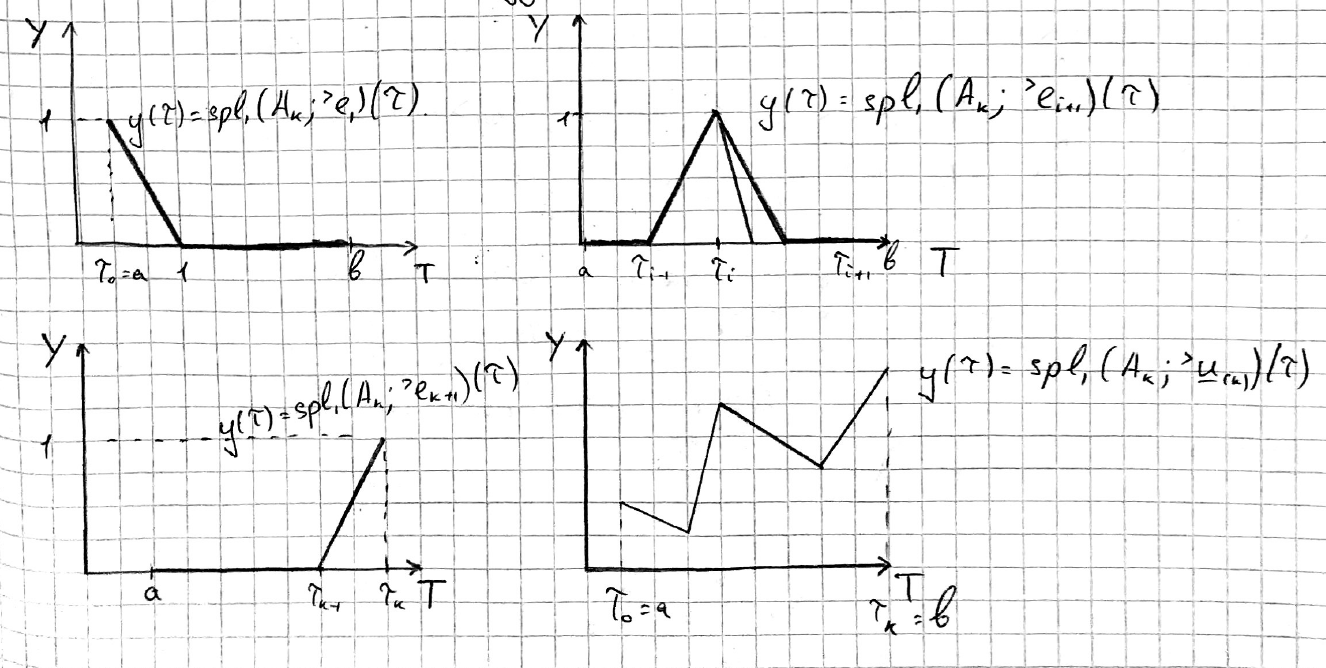
\includegraphics[width=0.7\linewidth]{img/img_9-1}
	\caption{}
	\label{img9-1}
\end{figure}

Следовательно, для $k \in \mathbb{N}$ определена интерпретация $\hat{\varphi}_k \in Hom \left(\underline{\upsilon}_{\left(k\right)},[H_k]\right)$:

$$
\hat{\varphi}_k \left({}^>\underline{U}_{\left(k\right)}\right) = \sum_{i=0}^k U_i spl_1 \left(A_k;{}^>e_{i+1}\right),
$$

то есть $\hat{\varphi}_k = \hat{H}_k - H_k$ - базисное отображение и $\| \hat{\varphi}_k \|=1$ для $k \in \mathbb{N} \left(\lim_{k\rightarrow + \infty} \| \varphi_k \| = 1\right)$.

В результате, для каждого $k \in \mathbb{N}$ определена аппроксимация $\hat{p}_k = \hat{\varphi}_k \circ \hat{A}_k \in Hom_c \left(Y_0;[H_k]\right)$ и $\| \hat{p}_k \| \leq \| \hat{\varphi}_k \| \cdot \| \hat{A}_k \| \leq 1$.

Поэтому аппроксимирование $\hat{p}_{\left(\cdot\right)} = \left(\hat{p}_k\right)_{\mathbb{N}}$ пространства $Y_0$ - устойчиво и аналитически корректно, то есть $\lim_{k\rightarrow + \infty} \hat{p}_k \left(y_0\right) = y_0$ для $\forall y_0 \in Y_0$. Следовательно, аппроксимирование $\hat{p}_{\left(\cdot\right)}$ - корректно.

\begin{figure}[h!]
	\centering
	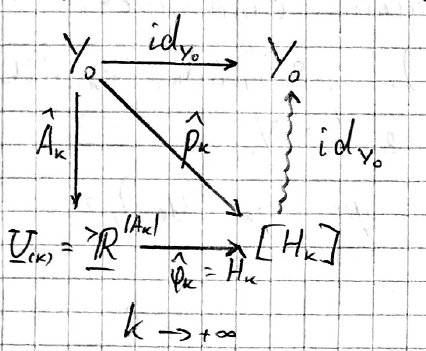
\includegraphics[width=0.4\linewidth]{img/img_9-2}
	\caption{}
	\label{img9-2}
\end{figure}

\paragraph{Пункт Б}

$$\overline{G} = [a;b] \times [c;d] = G \bigcup \partial G,$$

где $\partial G$ - граница $G$.

Пусть $A = \langle a = \tau_0, \tau_1,...,\tau_k \rangle$ - равномерная сетка $[a;b]$ и $stp \left(A\right) = \frac{b-a}{k} = \tau, B = \langle c = \theta_0, \theta_1,...,\theta_m \rangle$ - равномерная сетка $[c;d]$ шага $stp \left(B\right) = \frac{c-d}{m} = \theta$.

Сетка $C = A \times B = \{\left(\tau_i,\theta_j \right): i = \overline{0,k}, \ j = \overline{0,m} \}$.

\begin{figure}[h!]
	\centering
	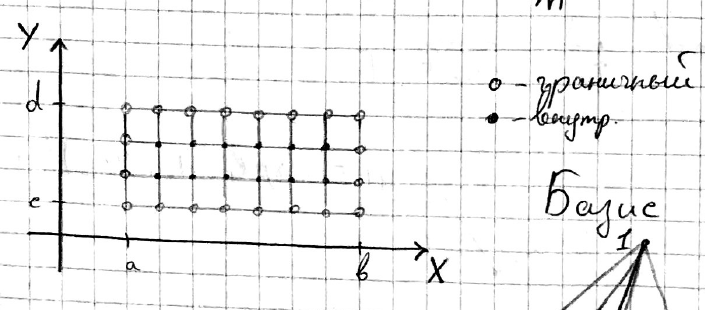
\includegraphics[width=0.4\linewidth]{img/img_9-3}
	\caption{}
	\label{fig:img9-3}
\end{figure}

\end{document}